% JuliaCon proceedings template
\documentclass{juliacon}
\setcounter{page}{1}
\usepackage{subcaption}
\usepackage{hyphenat}
\title{SemanticModels.jl}
\renewcommand{\theparagraph}{}
\newcommand{\semanticModels}{\nohyphens{\texttt{SemanticModels.jl}}}

\begin{document}

% **************GENERATED FILE, DO NOT EDIT**************

\title{SemanticModels.jl: A Julia Package for Scientific Model Augmentation}

\author[1]{Micah Halter}
\author[1]{Sreenath Raparti}
\author[1]{Kun Cao}
\author[1]{Christine Herlihy}
\author[1]{James Fairbanks}
\affil[1]{Georgia Tech Research Institute, Atlanta, USA}

\keywords{Modeling Frameworks, Meta-programming, Category Theory}



\maketitle

\begin{abstract}
\semanticModels{} is a package that takes advantage of meta-modeling and meta-programming to automate model augmentation and creation.
We chose Julia for our project because of the powerful type system, the efficient internal abstract syntax tree (AST), and the embedded domain specific languages (DSL) that emerge as a result through the multiple dispatch mechanism for all libraries in the Julia ecosystem~\cite{doi:11.1137/141000671}.
The dynamic type inference and method generation has significant and powerful downstream effects which enables dynamic model manipulation with efficient code generation.
These DSLs allow for strong theoretical category definitions and classifications of models to define conceptually sound universal rewrite rules for any given model class.
\end{abstract}

\section{Methodological Approach}\label{sec:body}
\paragraph{Introduction}\label{par:intro}
\semanticModels{} facilitates several metamodeling tasks by detecting and exploiting the implicit relationships between the semantically rich, natural language-based representations of scientific knowledge found in academic papers, and the relatively semantically sparse, but modular and precise representations found in code.
We provide a generalized model structure to support metamodeling tasks that may be exploratory, iterative, and/or inter-disciplinary in nature.
Our software can augment scientific workflows in support of a wide range of objectives, from model space exploration and hypothesis generation to model selection in complex workflows.

\paragraph{Language Selection}\label{par:julia}
Julia breaks the mold of other common scientific computing languages such as \texttt{R}, \texttt{Python}, and \texttt{MATLAB} by emphasizing features such as multiple dispatch and meta-programming.
Meta-programming is the ability to write programs that generate programs, usually, by representing code as a data structure within the program.
This facilitates more generalized routines to modify, generate, and transform programs.
Julia meta-programming is much easier than generating code for a static compiler, and because of the Julia just-in-time compiler, yields faster executions than a dynamic language like Python.

\paragraph{Model Augmentation}\label{par:model_augmentation}
The susceptible-infected-susceptible (SIS) model shown in Figure~\ref{fig:SIS} is one of the simplest models of infectious disease.
Susceptible individuals, $S$, are infected by infected individuals, $I$, at a per-capita rate $\beta I$, and infected individuals recover at a per-capita rate $\gamma$ to become susceptible again.
An extension of this model is the SIR model outlined in Figure~\ref{fig:SIR}, the SIR model adds a new state, $R$, for individuals that have recovered from their infection~\cite{epirecipes} and are no longer susceptible to new infections.
The core of functionality shown in Figure~\ref{fig:graft} ingesting and manipulating previously written modeling scripts. For example, taking a code that implements an SIS model and transforming it into an SIR model using meta-programming.
In the \texttt{model} function, the AST of a program is indexed for specific features that are known to be important for dynamical systems such as the states that the population can occupy, the rate relationships, and the state transition functions.
SemanticModels.jl captures the meaningful structures of a code with links to how a library defines a class of problems and enables high level program transformations that scientists recognise as \emph{perturbing the model}.
In Figure~\ref{fig:graft}, when we look at the programmatic replacement for the $dS$ term, the AST is searched for the definition of \texttt{dS}.
The \texttt{add} function takes in a newly defined state with a name, transition function, and initial value and places each of those components in the appropriate location within the AST.\@ The new model is solved by generating a new problem instance along with the necessary methods and calling the library solver functions.


\paragraph{Conclusion}\label{par:conclusion}
\semanticModels{} aims to leverage scientific knowledge currently trapped in the body of scientific code.
While open source code is a prerequisite for reproducible research, it is not sufficient towards understanding complex modeling code.
We present an automated system for extracting information from, reasoning about, and augmenting computational models.
This framework enables the extension of models with new parameters and components, leveraging the dynamic nature of the Julia compiler.

\begin{figure}[b]
  \begin{subfigure}[b]{0.16\textwidth}
    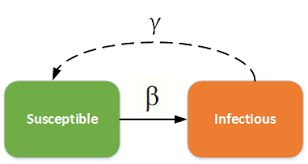
\includegraphics[width=\textwidth]{img/SIS.png}
    \caption{The flow of a SIS model.}\label{fig:SIS}
  \end{subfigure}
  \hspace{1em}
  \begin{subfigure}[b]{0.26\textwidth}
    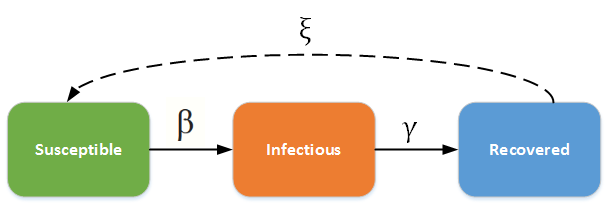
\includegraphics[width=\textwidth]{img/SIR-SIRS.png}
  \vspace{0em}
    \caption{The flow of a SIR model.}\label{fig:SIR}
  \end{subfigure}

\vspace{-1em}
\begin{subfigure}[b]{0.45\textwidth}
\begin{lstlisting}[language=Julia]
# read model into SemanticModels
sis = parsefile("epicookbook/src/SISModel.jl");
sis = model(ExpODEModel,sis);
# redefine a flux (rate) within the model
replace(sis.funcs[1],:dS,:(-β * S * I))
# define a new state and add it to our model
dR = Definition(:dR,:(γ * I),0)
sis.funcs[1] = add(sis.funcs[1],dR)
\end{lstlisting}
\caption{SIS to SIR using SemanticModels.jl}\label{fig:graft}
\end{subfigure}

\caption{An example of model manipulation.}
\end{figure}
% **************GENERATED FILE, DO NOT EDIT**************

\bibliographystyle{juliacon}
\bibliography{ref.bib}


\end{document}
% Inspired by the International Journal of Computer Applications template
